\documentclass{article}

\usepackage[utf8]{inputenc}
\usepackage[T1]{fontenc}
\usepackage[french]{babel}
\usepackage{amssymb}
\usepackage{graphicx}
\usepackage{ntheorem}
\usepackage{amsmath}
\usepackage{amssymb}
\usepackage[ a4paper, hmargin={3cm, 3cm}, vmargin={3cm, 3cm}]{geometry}

\usepackage{hyperref}
\hypersetup{
    colorlinks,
    citecolor=black,
    filecolor=black,
    linkcolor=blue,
    urlcolor=blue
}

\theoremstyle{plain}
\theorembodyfont{\normalfont}
\theoremseparator{~--}
\newtheorem*{define}{Définition}%[section]

\usepackage{tikz}
\usetikzlibrary{automata, positioning, arrows}
\usepackage{capt-of}

\usepackage{listings}
\definecolor{isarblue}{HTML}{006699}
\definecolor{isargreen}{HTML}{009966}
\definecolor{isarred}{HTML}{990066}
\lstdefinelanguage{isabelle}{%
    keywords=[1]{type_synonym,datatype,fun,abbreviation,definition,proof,typ,
                 term,lemma,theorem,corollary,unfolding},
    keywordstyle=[1]\bfseries\color{isarblue},
    keywords=[2]{where,assumes,shows,and},
    keywordstyle=[2]\bfseries\color{isargreen},
    keywords=[3]{if,then,else,case,of,SOME,let,in,O},
    keywordstyle=[3]\color{isarblue},
    keywords=[4]{apply,done},
    keywordstyle=[4]\color{isarred}
}
\lstset{%
  language=isabelle,
  escapeinside={&}{&},
  columns=fixed,
  extendedchars,
  basewidth={0.5em,0.45em},
  basicstyle=\ttfamily,
  captionpos=b,
  mathescape,
}

\title{Rapport TP1}
\author{Valeran MAYTIE}
\date{}

\begin{document}
  \maketitle

  \section{Prise en main du logiciel Isabelle}

  On a commencé par utiliser 2 commandes :

  \begin{itemize}
    \item \texttt{typ}  : détermine si un type est bien formé.
    \item \texttt{term} : détermine si un term est bien formé et donne son type
      s'il est typable le plus général (Algo W).
  \end{itemize}

  D'abord, on a écrit des types bien formés par exemple :

  \begin{lstlisting}
typ $\langle$int $\Rightarrow$ int$\rangle$
typ $\langle$'$\alpha$ list $\Rightarrow$ '$\beta$ set$\rangle$
  \end{lstlisting}

  Ensuite, on a écrit des termes. Grâce à l'algorithme W implémenté dans
  Isabelle, on peut obtenir le type le plus général des termes écrits.

  Pour débuter, on a écrit deux termes assez simples :

  \begin{lstlisting}
term $\langle$$\lambda$x. x$\rangle$
term $\langle$[1, 2, 3::nat]$\rangle$
  \end{lstlisting}

  Le \texttt{::nat} dans le deuxième terme sert à spécifier le type contenu dans
  la liste. Si cette spécification n'est pas faite l'algorithme nous sortira le
  type \texttt{'$\alpha$ list}. Les symboles $1$, $2$ et $3$ ne sont pas des
  entiers, mais des types généraux : $'\alpha$ (Pour garder la possibilité de
  redéfinir ces symboles).

  L'éditeur de texte à une super fonctionnalité qui permet d'afficher les
  fichiers de définition. Il suffit de faire un \texttt{Ctrl+clic droit} sur la
  définition voulue.

  On peut écrire des termes assez compliqués comme celui-ci :

\begin{lstlisting}
term $\langle$($\lambda$x. $\lambda$y. ($\lambda$z.($\lambda$x. z x) ($\lambda$y. z y)) (x y))$\rangle$
\end{lstlisting}

  Isabelle le rejet, car il ne peut pas être typé. En réalité ce terme cache une
  auto application. Il se réduit en :
  $\lambda x\;y.\;(x\;y)\;(\lambda z.\; (x\;y)\;z)$. Or ce genre
  de $\lambda$-term ne sont pas acceptés par le système de type $\lambda2$
  (polymorphisme).

  On récupère dans la console l'erreur :
  \begin{center}
    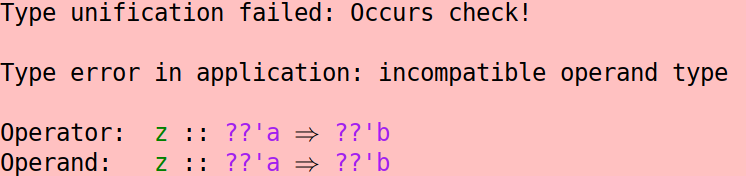
\includegraphics[scale=0.5]{error.png}
  \end{center}

  Pour débuger un terme comme celui-ci, on peut remplacer la variable par une
  variable libre en mettant une apostrophe après. On peut remarquer que les
  variables libres sont coloriées en bleu dans l'interface.

  \section{Axiome}
    Dans une théorie logique, on va parfois utiliser des axiomes, car certains
    énoncés jugé correct ne sont pas prouvables. Par exemple le tiers exclu ($u
    \vee \neg u$) n'est pas prouvable dans les logiques constructives. Pour
    cella en Isabelle, on peut ajouter des axiomes qui sont des énoncés acceptés
    par le c\oe{}ur d'Isabelle sans preuve. Il faut donc bien faire attention
    avant d'ajouter ce genre d'énoncé, car accepter un axiome faux va mettre à
    malle toute la cohérence d'Isabelle.

    Par exemple dans le TP, on nous demande de rajouter l'axiome du combinateur
    de point fixe :

    $$\forall f,\;\exists Y,\; Y\;f = f\;(Y\;f)$$

    Malheureusement cette formule est fausse. Si on applique cette formule à $f
    = \neg := \lambda x. \bot$ on obtient $Y\;\neg = \neg\;(Y\;\neg)$ ce qui
    n'est pas vrai.

    Un tel $\lambda$-terme existe $\lambda f.\;(\lambda x.\;f\;(x\;x))\;
    (\lambda x.\;f\;(x\;x))$, mais il n'est pas typable, il est alors refusé par
    Isabelle.

  \section{Encodage de Church}
    On cherche à encoder les entiers naturels en $\lambda$-calcul pur. Pour cela
    on utilise l'encodage de Church, il est construit avec une fonction qui
    prend en paramètre deux variables $f$ une fonction et $x$ une variable. Pour
    représenter un nombre $n$ on compose $n$ fois la fonction $f$ appliquée
    à $x$.

    Le $\lambda$-term ressemble à :
    $$
      \lambda f.\lambda x. f^n\;x \equiv 
      \lambda f.\lambda x.\;\underbrace{f\;(f\;\ldots\;(f}_{n\text{ fois}}\; x))
    $$

    En Isabelle nous définissons les entiers naturels de 0 à 5 comme ceci :

    \begin{figure}[thpb]
    \begin{lstlisting}
definition ZERO  where "ZERO  $\equiv$ $\lambda$f x. x "
definition ONE   where "ONE   $\equiv$ $\lambda$f x. f x"
definition TWO   where "TWO   $\equiv$ $\lambda$f x. f (f x)"
definition THREE where "THREE $\equiv$ $\lambda$f x. f (f (f x))"
definition FOUR  where "FOUR  $\equiv$ $\lambda$f x. f (f (f (f x)))"
definition FIVE  where "FIVE  $\equiv$ $\lambda$f x. f (f (f (f (f x))))"
    \end{lstlisting}
    \caption{Entier de Church de 0 à 5}
    \label{fig:number}
    \end{figure}

    On peut définir des opérations sur cet encodage.

  \begin{center}
    \begin{tabular}{r c l}
      $n + 1$      & : & $\lambda n\;f\;x.\;f (n\;f\;x)$          \\
      $n + m$      & : & $\lambda n\; m\;f\;x.\;m\; f\;(n\;f\;x)$ \\
      $n \times m$ & : & $\lambda n\; m\;f\;x.\;n\;(m\;f)\;x$     \\
      $n^m$        & : & $\lambda n\; m\;f\;x.\;m\; n$            \\
    \end{tabular}
  \end{center}

  Malheureusement les opérations prédécesseur et soustraction sont plus
  difficiles à écrire.

  En Isabelle, on définit uniquement l'addition (Figure-\ref{fig:add}) car ça
  sera la seule utile pour notre première preuve.

    \begin{figure}[thpb]
    \begin{lstlisting}
definition PLUS where "PLUS $\equiv$ $\lambda$n m f x. m f (n f x)"
    \end{lstlisting}
    \caption{Addition avec l'encodage de Church}
    \label{fig:add}
    \end{figure}

  Notre première démonstration consiste à prouver que $3 + 2 = 5$ en entier
  de Church. L'énoncé s'écrit comme ceci : \texttt{PLUS TWO THREE = FIVE}.
  Pour commencer, il faut dérouler toutes les définitions.
  On utilise donc la tactique \texttt{unfolding} avec comme argument la
  définition à déplier suivit de ``\textit{\_def}'' (par exemple pour la
  définition \textit{PLUS} : \textit{PLUS\_def}).

  Le dépliage va effectuer tous les calculs possibles, on aura donc :
  $$
  \texttt{PLUS TWO THREE }\to^*_\beta\;\lambda f\; x.\;f\;(f\;(f\;(f\;(f\;x))))
  $$

  Nous remarquons que \texttt{PLUS TWO THREE} se réduit en \texttt{FIVE}, il
  nous reste à monter que \texttt{FIVE = FIVE}.
  Nous avons vu en cours que l'égalité de Isabelle est réflexive
  ($\forall x, x = x$). Il suffit d'appliquer le théorème de réflexivité
  \textit{HOL.refl} que l'on peut trouver à l'aide de la commande
  \texttt{find\_theorems "\_ = \_"}. On peut appliquer ce théorème en utilisant
  \texttt{apply(rule refl)}. La preuve complète de deux lignes :) se trouve
  ci-dessous (Figure-\ref{fig:preuve}).

    \begin{figure}[htb]
    \begin{lstlisting}
lemma the_first : "PLUS TWO THREE = FIVE"
  unfolding PLUS_def TWO_def THREE_def FIVE_def
  apply(rule refl)
  done
    \end{lstlisting}
    \caption{Preuve que $2 + 3 = 5$ avec l'encodage de Church}
    \label{fig:preuve}
    \end{figure}

    Une fois que tous les buts sont prouvés, on a le message suivant indiquant
    que la preuve est finie :
    \begin{center}
      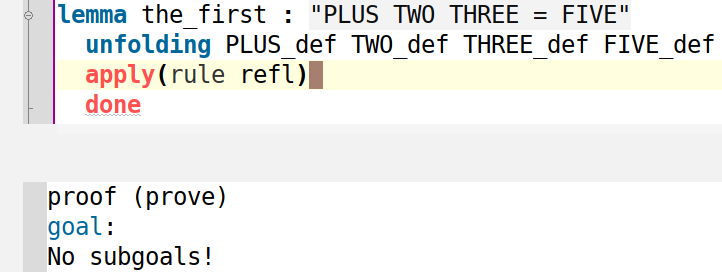
\includegraphics[scale=0.3]{fin_preuve.png}
    \end{center}

    Les théorèmes prouvés sont rajoutés au c\oe{}r d'Isabelle. On peut afficher
    l'énoncé du théorème en utilisant la commande \texttt{thm \textit{nom}}.
    Elle va afficher l'énoncé du théorème \textit{nom} dans la console.

\end{document}
